\chapter{Project dipole radiation onto nanofiber modes: far field approximation (a rough model)}\label{ch:FreeDipoleProjection}
As a trial, we only add one atom in the nanofiber-trapped-atoms system. 
Considering the detector is far away from the atom compared to the distance between the atom and the nanofiber, the paraxial approximation\index{paraxial approximation} holds for our case where our measurement on the optical field is applied after a distant transmission through the fiber. \textcolor{red}{We also assume that the emission from the atom propagates in free space by vanishing the boundary condition defined by the nanofiber, so that we can use the conclusion of the Green function for free space. }
The scattered optical field can be written as 
\begin{align}
\boldsymbol{\mathcal{E}}^s(\br) &=-k_0^2\left(\boldsymbol{\alpha}\cdot \boldsymbol{\mathcal{E}}^g(\br')\right)_\perp \frac{e^{ik_0 \left| \br-\br' \right| }}{\left| \br-\br'\right| }\\
&=-k_0^2\left[ \boldsymbol{\alpha}\!\cdot\! \boldsymbol{\mathcal{E}}^g(\br') - \left(\hat{\mathrm{r}}\! \cdot\! \boldsymbol{\alpha}\!\cdot\! \boldsymbol{\mathcal{E}}^g(\br') \right) \hat{\mathrm{r}}\right] \frac{e^{ik_0 \left| \br-\br' \right| }}{\left| \br-\br'\right| }\\
&\approx -k_0^2\left[ \boldsymbol{\alpha}\!\cdot\! \boldsymbol{\mathcal{E}}^g(\br') - \left(\hat{\mathrm{e}}_z\! \cdot\! \boldsymbol{\alpha}\!\cdot\! \boldsymbol{\mathcal{E}}^g(\br') \right) \hat{\mathrm{e}}_z\right] \frac{e^{ik_0 \left| \br-\br' \right| }}{\left| \br-\br'\right| }\\
&=-k_0^2 \left[\left(\hat{\mathrm{e}}_{r_\perp} \! \cdot \! \boldsymbol{\alpha} \! \cdot\! \boldsymbol{\mathcal{E}}^g(\br')\right)\hat{\mathrm{e}}_{r_\perp} + \left(\hat{\mathrm{e}}_\phi \! \cdot \! \boldsymbol{\alpha} \! \cdot \! \boldsymbol{\mathcal{E}}^g(\br') \right)\hat{\mathrm{e}}_\phi \right] 
\frac{e^{ik_0 \left| \br-\br' \right| }}{\left| \br-\br'\right| }\\
&\approx \frac{-k_0^2 e^{ik_0(z\!-\!z'\!)}}{z\!-\!z'}\left[\left(\hat{\mathrm{e}}_{r_\perp} \!\!\cdot\! \boldsymbol{\alpha}\!\cdot\! \boldsymbol{\mathcal{E}}^g(\br')\right)\hat{\mathrm{e}}_{r_\perp} \!\! +\! \left(\hat{\mathrm{e}}_\phi\!\cdot\! \boldsymbol{\alpha}\!\cdot\! \boldsymbol{\mathcal{E}}^g(\br') \right)\hat{\mathrm{e}}_\phi \right] \exp\!\! \left[ \frac{ik_0 \left| \mathrm{r}_\perp\! - \mathrm{r}_\perp'\right|}{2(z-z')}  \right],\label{Erscatt}
\end{align}
where $ \boldsymbol{\alpha} $ is the polarizability tensor only depending on the internal state of the atom; $ \left| \mathrm{r}_\perp - \mathrm{r}_\perp'\right|=\sqrt{r_\perp^2+{r_\perp'}^2 - 2 r_\perp r_\perp'\cos(\phi-\phi')} $ where $ (r_\perp',\phi',z') $ is the coordinate of the atom. 

As shown in Equ.~\ref{Erscatt}, the scattered field does not have a $ z $-component in the far field by using a free space Green function. 

We can decompose the guided mode into left- and right-handed circular fundamental modes using Equ.~\ref{Eilincyc}. For instance, if the incident light is $ x $-polarized (horizontally polarized) with the normalized field $ \boldsymbol{\mathcal{E}}^g (\br)=\boldsymbol{\mathcal{E}}_H (\br) $, and $ \mathbf{E}^g (\br,t) = \boldsymbol{\mathcal{E}}_H(\br)e^{-i\omega t} $ is a forward propagating light, we can use the relationship that
\begin{subequations}
\label{ErPMHV}
\begin{align}
\boldsymbol{\mathcal{E}}^+ &= \frac{1}{\sqrt{2}} \left(\boldsymbol{\mathcal{E}}_H+i\boldsymbol{\mathcal{E}}_V \right),\\
\boldsymbol{\mathcal{E}}^- &= \frac{1}{\sqrt{2}} \left( \boldsymbol{\mathcal{E}}_H-i\boldsymbol{\mathcal{E}}_V \right),
\end{align}
\end{subequations}
where $ \boldsymbol{\mathcal{E}}_V $ is the normalized mode with a $ y $-polarized (vertically polarized) incident light which is orthogonal to $ \boldsymbol{\mathcal{E}}_H $. Based on Equ.~\ref{ErPMHV}, we can solve for $ \boldsymbol{\mathcal{E}}_H $ to give
\begin{align}
\boldsymbol{\mathcal{E}}_H &= \frac{1}{\sqrt{2}} \left(\boldsymbol{\mathcal{E}}^+ + \boldsymbol{\mathcal{E}}^- \right),\\
\boldsymbol{\mathcal{E}}_V &= \frac{i}{\sqrt{2}} \left( \boldsymbol{\mathcal{E}}^- -\boldsymbol{\mathcal{E}}^+ \right). 
\end{align}
Therefore, the spatial dependent scattered electrical field can be given by
\begin{align}
\boldsymbol{\mathcal{E}}^s(\br) &\approx  \frac{-\!k_0^2 e^{ik_0(z\!-\!z'\!)}}{z\!-\!z'}\! \left[\left(\hat{\mathrm{e}}_{r_\perp} \!\!\cdot\! \boldsymbol{\alpha}\!\cdot\! \boldsymbol{\mathcal{E}}_H(\br')\right)\hat{\mathrm{e}}_{r_\perp} \!\!  +\! \left(\hat{\mathrm{e}}_\phi\!\cdot\! \boldsymbol{\alpha}\!\cdot\! \boldsymbol{\mathcal{E}}_H(\br') \right)\hat{\mathrm{e}}_\phi \right] \exp\!\! \left[ \frac{ik_0 \left| \mathrm{r}_\perp\!\! -\! \mathrm{r}_\perp'\right|}{2(z-z')}  \right]\\
&= - \frac{k_0^2 e^{ik_0(z\!-\!z'\!)}}{\sqrt{2}(z\!-\!z')} \left(\hat{\mathrm{e}}_{r_\perp} \!\!\cdot\! \boldsymbol{\alpha}\!\cdot\! \left(\boldsymbol{\mathcal{E}}^+ (\br') \!\! +\! \boldsymbol{\mathcal{E}}^- (\br') \right)\right)\hat{\mathrm{e}}_{r_\perp}  \exp\!\! \left[ \frac{ik_0 \left| \mathrm{r}_\perp\!\! -\! \mathrm{r}_\perp'\right|}{2(z-z')}  \right] \nonumber\\
&\qquad - \frac{k_0^2 e^{ik_0(z\!-\!z'\!)}}{\sqrt{2}(z\!-\!z')} \left(\hat{\mathrm{e}}_{\phi} \!\!\cdot\! \boldsymbol{\alpha}\!\cdot\! \left(\boldsymbol{\mathcal{E}}^+ (\br') \!\! +\! \boldsymbol{\mathcal{E}}^- (\br') \right)\right)\hat{\mathrm{e}}_{\phi}  \exp\!\! \left[ \frac{ik_0 \left| \mathrm{r}_\perp\!\! -\! \mathrm{r}_\perp'\right|}{2(z-z')}  \right]. \label{Ers0}
\end{align}
Using Equs.~\ref{Ertcrla} and~\ref{Ertcrga}, the $ \boldsymbol{\mathcal{E}}_H (\br')= \boldsymbol{\mathcal{E}}^+ (\br') \!\! +\! \boldsymbol{\mathcal{E}}^- (\br') $ is given by
\begin{subequations}
\label{EHrcrla}
\begin{align}
{\mathcal{E}_H}_{r_\perp} (\br') &= A\frac{\beta_{11}}{h_{11}}\nonumber\\
&\qquad \left[ (1\!-\!s_{11})J_0(h_{11}r'_\perp)\!-\! (1\!+\!s_{11})J_2(h_{11}r_\perp') \right]e^{if\beta_{11} z'}\cos{\phi'}\\
{\mathcal{E}_H}_\phi(\br') &=  iA \frac{\beta_{11}}{2h_{11}} \nonumber\\
&\qquad \left[ (1\!-\!s_{11})J_0(h_{11}r'_\perp)\! +\! (1\!+\!s_{11})J_2(h_{11}r'_\perp) \right] e^{if\beta_{11} z' }\sin(\phi')\\
{\mathcal{E}_H}_z(\br') &= i2A J_1(h_{11}r'_\perp) e^{if\beta_{11} z'}\cos(\phi')
\end{align}
\end{subequations}
for $ r'_\perp<a $, and by
\begin{subequations}
\label{EHrpcrga}
\begin{align}
{\mathcal{E}_H}_{r_\perp}(\br') &=A\frac{\beta_{11}}{h_{11}}\frac{J_1(h_{11}a)}{K_1(q_{11}a)}\nonumber\\ 
&\qquad \left[ (1\!-\!s_{11})K_0(q_{11}r'_\perp)\!+\!(1 \!+\! s_{11})K_2(q_{11}r'_\perp) \right]e^{if\beta_{11} z' }\cos(\phi')\\
{\mathcal{E}_H}_\phi(\br') &=  iA \frac{\beta_{11}}{h_{11}} \frac{J_1(h_{11}a)}{K_1(q_{11}a)}\nonumber\\ 
&\qquad \left[ (1\!-\!s_{11})K_0(q_{11}r'_\perp) \! -\! (1\!+\!s_{11})K_2(q_{11}r'_\perp) \right] e^{if\beta_{11} z'}\sin(\phi')\\
{\mathcal{E}_H}_z(\br') &= i2A \frac{J_1(h_{11}a)}{K_1(q_{11}a)} K_1(q_{11}r'_\perp) e^{if\beta_{11} z'}\cos(\phi')
\end{align}
\end{subequations}
for $ r'_\perp>a $. We define $ \mathbf{T}^{f}(\br')= \boldsymbol{\alpha}\!\cdot \boldsymbol{\mathcal{E}}_H (\br') = \boldsymbol{\alpha}\!\cdot\! \left(\boldsymbol{\mathcal{E}}^+ (\br') \!\! +\! \boldsymbol{\mathcal{E}}^- (\br') \right) $, which is a constant vector, and only the $ r_\perp $ and $ \phi $ components contribute to the scattered field in the far field. Now, Equ.~\ref{Ers0} can be rewritten as
\begin{align}
\boldsymbol{\mathcal{E}}^s(\br) &=- \frac{k_0^2 e^{ik_0(z\!-\!z'\!)}}{\sqrt{2}(z\!-\!z')} \exp\!\! \left[ \frac{ik_0 \left| \mathrm{r}_\perp\!\! -\! \mathrm{r}_\perp'\right|}{2(z-z')}  \right]\! \left[ T_{r_\perp}^f(\br') \hat{\mathrm{e}}_{r_\perp} \! + T^f_\phi (\br') \hat{\mathrm{e}}_{\phi} \right],
\end{align}
where $ T^f_{r_\perp}(\br') $ and $ T^f_\phi (\br') $ are the $ r_\perp $ and $ \phi $ components of $ \mathbf{T}^f(\br')$. 

The total electrical field can be written as 
\begin{align}
\boldsymbol{\mathcal{E}}(\br) &= \boldsymbol{\mathcal{E}}^g(\br) + \boldsymbol{\mathcal{E}}^s(\br)\\
&\approx  \frac{1}{\sqrt{2}} \left(\boldsymbol{\mathcal{E}}^+(\br)\!\! +\! \boldsymbol{\mathcal{E}}^-(\br) \right) \nonumber\\
&\qquad - \frac{k_0^2 e^{ik_0(z\!-\!z'\!)}}{\sqrt{2}(z\!-\!z')} \left(\hat{\mathrm{e}}_{r_\perp} \!\!\cdot\! \boldsymbol{\alpha}\!\cdot\! \left(\boldsymbol{\mathcal{E}}^+ (\br') \!\! +\! \boldsymbol{\mathcal{E}}^- (\br') \right)\right)\hat{\mathrm{e}}_{r_\perp}  \exp\!\! \left[ \frac{ik_0 \left| \mathrm{r}_\perp\!\! -\! \mathrm{r}_\perp'\right|}{2(z-z')}  \right] \nonumber\\
&\qquad - \frac{k_0^2 e^{ik_0(z\!-\!z'\!)}}{\sqrt{2}(z\!-\!z')} \left(\hat{\mathrm{e}}_{\phi} \!\!\cdot\! \boldsymbol{\alpha}\!\cdot\! \left(\boldsymbol{\mathcal{E}}^+ (\br') \! +\! \boldsymbol{\mathcal{E}}^- (\br') \right)\right)\hat{\mathrm{e}}_{\phi}  \exp\!\! \left[ \frac{ik_0 \left| \mathrm{r}_\perp\!\! -\! \mathrm{r}_\perp'\right|}{2(z-z')}  \right]\\
&= \frac{1}{\sqrt{2}} \boldsymbol{\mathcal{E}}_H(\br)  \!-\! \frac{k_0^2 e^{ik_0(z\!-\!z'\!)}}{\sqrt{2}(z\!-\!z')} \exp\!\! \left[ \frac{ik_0\! \left| \mathrm{r}_\perp\!\! -\! \mathrm{r}_\perp'\right|}{2(z-z')}  \right]\!\! \left[ T^f_{r_\perp}(\br') \hat{\mathrm{e}}_{r_\perp} \!\! +\! T^f_\phi (\br') \hat{\mathrm{e}}_{\phi} \right].
\end{align}
%where $ \eye $ is the unitary diagonal tensor. Now, we can see that the total optical field strongly depends on the bound field and the polarization of the atom.

To further discuss how backward and forward scattering contribute to the bound mode, we consider both the space- and time-dependent electrical field of the scattered contribution $ \mathbf{E}^s(\br,t) $, and project it to the normalized forwarded and backwarded bound modes.  In principle, we can decompose the scattered electrical field as 
\begin{align}
\mathbf{E}^s(\br,t) =\sum_\mu C^{(\mu)}(z) \mathbf{E}^{(\mu)} (\br,t),
\end{align}
with
\begin{align}
C^{(\mu)} (z) = \int_0^{2\pi}\mathrm{d}\phi \int_0^\infty {\mathbf{E}^{(\mu)}}^* (\br,t) \cdot \mathbf{E}^s(\br,t)r_\perp \mathrm{d}r_\perp.
\end{align}

For the Green function we used above, the coefficients in the far field can be calculated as
\begin{align}
C^{(\mu)} (z) &= - \frac{k_0^2 T^{f'}_{r_\perp}(\br') e^{ik_0(z\!-\!z'\!)}}{\sqrt{2}(z\!-\!z')}\int_0^{2\pi}\mathrm{d}\phi \int_0^\infty {\mathcal{E}^{(\mu)}_{r_\perp}}^* (\br) \exp\!\! \left[ \frac{ik_0 \left| \mathrm{r}_\perp\!\! -\! \mathrm{r}_\perp'\right|}{2(z-z')}  \right]\!  r_\perp \mathrm{d}r_\perp \nonumber\\
&\quad - \frac{k_0^2 T^{f'}_\phi(\br') e^{ik_0(z\!-\!z'\!)} }{\sqrt{2}(z\!-\!z')}\int_0^{2\pi}\mathrm{d}\phi \int_0^\infty {\mathcal{E}^{(\mu)}_\phi}^* (\br) \exp\!\! \left[ \frac{ik_0 \left| \mathrm{r}_\perp\!\! -\! \mathrm{r}_\perp'\right|}{2(z-z')}  \right]\!  r_\perp \mathrm{d}r_\perp \\
&=  - \frac{k_0^2 T^{f'}_{r_\perp}(\br') e^{ik_0(z\!-\!z'\!)}}{\sqrt{2}(z\!-\!z')}\int_0^{2\pi}\mathrm{d}\phi \int_0^a {\mathcal{E}^{(\mu)}_{r_\perp}}^* (\br) \exp\!\! \left[ \frac{ik_0 \left| \mathrm{r}_\perp\!\! -\! \mathrm{r}_\perp'\right|}{2(z-z')}  \right]\!  r_\perp \mathrm{d}r_\perp \nonumber\\
&\quad - \frac{k_0^2 T^{f'}_{r_\perp}(\br') e^{ik_0(z\!-\!z'\!)}}{\sqrt{2}(z\!-\!z')}\int_0^{2\pi}\mathrm{d}\phi \int_a^\infty {\mathcal{E}^{(\mu)}_{r_\perp}}^* (\br) \exp\!\! \left[ \frac{ik_0 \left| \mathrm{r}_\perp\!\! -\! \mathrm{r}_\perp'\right|}{2(z-z')}  \right]\!  r_\perp \mathrm{d}r_\perp \nonumber\\
&\quad - \frac{k_0^2 T^{f'}_\phi(\br') e^{ik_0(z\!-\!z'\!)}}{\sqrt{2}(z\!-\!z')}\int_0^{2\pi}\mathrm{d}\phi \int_0^a {\mathcal{E}^{(\mu)}_\phi}^* (\br) \exp\!\! \left[ \frac{ik_0 \left| \mathrm{r}_\perp\!\! -\! \mathrm{r}_\perp'\right|}{2(z-z')}  \right]\!  r_\perp \mathrm{d}r_\perp \nonumber\\
&\quad - \frac{k_0^2 T^{f'}_\phi(\br') e^{ik_0(z\!-\!z'\!)}}{\sqrt{2}(z\!-\!z')}\int_0^{2\pi}\mathrm{d}\phi \int_a^\infty {\mathcal{E}^{(\mu)}_\phi}^* (\br) \exp\!\! \left[ \frac{ik_0 \left| \mathrm{r}_\perp\!\! -\! \mathrm{r}_\perp'\right|}{2(z-z')}  \right]\!  r_\perp \mathrm{d}r_\perp \\
&= - \frac{k_0^2 T^{f'}_{r_\perp}(\br') e^{ik_0(z\!-\!z'\!)\!-\!if\beta_{11} z}}{\sqrt{2}(z\!-\!z')}  \!\!\! \int_0^{2\pi}\!\!\! \mathrm{d}\phi \!\!\! \int_0^a   \mathcal{E}^{(\mu)}_{r_\perp}(r_\perp) e^{-i p\phi} 
\exp\!\! \left[ \frac{ik_0 \left| \mathrm{r}_\perp\!\! -\! \mathrm{r}_\perp'\right|}{2(z-z')}  \right]\!  r_\perp \mathrm{d}r_\perp \nonumber\\
&\quad - \frac{k_0^2 T^{f'}_{r_\perp}(\br') e^{ik_0(z\!-\!z'\!)\!-\!if\beta_{11} z}}{\sqrt{2}(z\!-\!z')}  \!\!\! \int_0^{2\pi}\!\!\! \mathrm{d}\phi \!\!\! \int_a^\infty \!\!\! {\mathcal{E}^{(\mu)}_{r_\perp}} (r_\perp) e^{-i p\phi} \exp\!\! \left[ \frac{ik_0 \left| \mathrm{r}_\perp\!\! -\! \mathrm{r}_\perp'\right|}{2(z-z')}  \right]\!  r_\perp \mathrm{d}r_\perp \nonumber\\
&\quad - \frac{k_0^2 T^{f'}_\phi(\br') e^{ik_0(z\!-\!z'\!)\!-\!if\beta_{11} z}}{\sqrt{2}(z\!-\!z')} \!\!\! \int_0^{2\pi}\!\!\! \mathrm{d}\phi \!\!\! \int_0^a \!\!\! {\mathcal{E}^{(\mu)}_\phi} (r_\perp) e^{-i p\phi} \exp\!\! \left[ \frac{ik_0 \left| \mathrm{r}_\perp\!\! -\! \mathrm{r}_\perp'\right|}{2(z-z')}  \right]\!  r_\perp \mathrm{d}r_\perp \nonumber\\
&\quad - \frac{k_0^2 T^{f'}_\phi(\br') e^{ik_0(z\!-\!z'\!)\!-\!if\beta_{11} z}}{\sqrt{2}(z\!-\!z')}  \!\!\! \int_0^{2\pi}\!\!\!\mathrm{d}\phi\!\!\!  \int_a^\infty \!\!\! {\mathcal{E}^{(\mu)}_\phi} (r_\perp) e^{-i p\phi} \exp\!\! \left[ \frac{ik_0 \left| \mathrm{r}_\perp\!\! -\! \mathrm{r}_\perp'\right|}{2(z-z')}  \right]\!  r_\perp \mathrm{d}r_\perp \\
&=  - \frac{k_0^2 T^{f'}_{r_\perp}(\br') e^{ik_0(z\!-\!z'\!)\!-\!if\beta_{11} z}}{\sqrt{2}(z\!-\!z')} \!\! \int_0^{2\pi}\!\!\! \mathrm{d}\phi \!\! \int_0^a  \!\! \mathcal{E}^{(\mu)}_{r_\perp}(r_\perp)  
\exp\!\! \left[ \frac{ik_0 \left| \mathrm{r}_\perp\!\! -\! \mathrm{r}_\perp'\right|}{2(z-z')} \!-\! i p\phi  \right]\!  r_\perp \mathrm{d}r_\perp \nonumber\\
&\quad - \frac{k_0^2 T^{f'}_{r_\perp}(\br') e^{ik_0(z\!-\!z'\!)\!-\!if\beta_{11} z}}{\sqrt{2}(z\!-\!z')}  \!\!\! \int_0^{2\pi}\!\!\!\mathrm{d}\phi \!\!\! \int_a^\infty \!\!\! {\mathcal{E}^{(\mu)}_{r_\perp}} (r_\perp)  \exp\!\! \left[ \frac{ik_0 \left| \mathrm{r}_\perp\!\! -\! \mathrm{r}_\perp'\right|}{2(z-z')} \!-\! i p\phi \right]\!  r_\perp \mathrm{d}r_\perp \nonumber\\
&\quad - \frac{k_0^2 T^{f'}_\phi(\br') e^{ik_0(z\!-\!z'\!)\!-\!if\beta_{11} z}}{\sqrt{2}(z\!-\!z')} \!\!\! \int_0^{2\pi} \!\!\! \mathrm{d}\phi \!\!\! \int_0^a\!\!\! {\mathcal{E}^{(\mu)}_\phi} (r_\perp) \exp\!\! \left[ \frac{ik_0 \left| \mathrm{r}_\perp\!\! -\! \mathrm{r}_\perp'\right|}{2(z-z')} \!-\! i p\phi \right]\!  r_\perp \mathrm{d}r_\perp \nonumber\\
&\quad - \frac{k_0^2 T^{f'}_\phi(\br') e^{ik_0(z\!-\!z'\!)\!-\!if\beta_{11} z}}{\sqrt{2}(z\!-\!z')}  \!\!\! \int_0^{2\pi}\!\!\! \mathrm{d}\phi \!\!\! \int_a^\infty \!\!\! {\mathcal{E}^{(\mu)}_\phi} (r_\perp) \exp\!\! \left[ \frac{ik_0 \left| \mathrm{r}_\perp\!\! -\! \mathrm{r}_\perp'\right|}{2(z-z')} \!-\! i p\phi \right]\!  r_\perp \mathrm{d}r_\perp. \label{Cmu1}
\end{align}
Using the relationship that $ \left| \mathrm{r}_\perp - \mathrm{r}_\perp'\right|=\sqrt{r_\perp^2+{r_\perp'}\!\!^2 - 2 r_\perp r_\perp'\cos(\phi-\phi')} $, the integral over $ \phi $ can be separated as 
\begin{align}
C^{(\mu)}_0(r_\perp,z) &= \int_0^{2\pi} \!\!\! \mathrm{d}\phi  \exp\!\! \left[ \frac{ik_0 \left| \mathrm{r}_\perp\!\! -\! \mathrm{r}_\perp'\right|}{2(z-z')} \!-\! i p\phi \right]\\
&= \int_0^{2\pi} \!\!\! \mathrm{d}\phi  \exp\!\! \left[ \frac{ik_0 \sqrt{r_\perp^2+{r_\perp'}\!\!^2 - 2 r_\perp r_\perp'\cos(\phi-\phi')} }{2(z-z')} \!-\! i p\phi \right]\\
&= \int_0^{2\pi} \!\!\! \mathrm{d}\phi  \exp\!\! \left[ \frac{ik_0 \sqrt{r_\perp^2 \!+ {r_\perp'}\!\!^2}\sqrt{1 \!-\! \frac{2 r_\perp r_\perp'}{r_\perp^2 \!+ {r_\perp'}\!\!^2}\cos(\phi \!-\! \phi')} }{2(z-z')} \!-\! i p\phi \right].
\end{align}
Calculating this integration analytically is not trivial unless $ r_\perp=r_\perp' $ or $ \br_\perp $ parallel to $ \br_\perp' $. We can calculate the projection coefficients numerically instead. Equ.~\ref{Cmu1} can be rewritten as
\begin{align}
C^{(\mu)} (z) &= - \frac{k_0^2 e^{ik_0(z\!-\!z'\!)\!-\!if\beta_{11} z} }{\sqrt{2}(z\!-\!z')}\left[  T^{f'}_{r_\perp}(\br') \mathcal{C}_{r_\perp}^p (z) +  T^{f'}_\phi(\br') \mathcal{C}_{\phi}^p(z) \right]\\
&= T^{f'}_{r_\perp}(\br') \mathcal{S}_{r_\perp}^p (z) +  T^{f'}_\phi(\br') \mathcal{S}_{\phi}^p(z),
\end{align}
where $ \mathcal{C}_{r_\perp}^p(z) $ and $ \mathcal{C}_\phi^p(z) $ correspond to the integrals with $ \mathcal{E}^{(\mu)}_{r_\perp} $ and $ \mathcal{E}^{(\mu)}_{\phi} $, repectively; Correspondingly, $ \mathcal{S}_{r_\perp}^p(z)=\mathcal{A}(z)\mathcal{C}_{r_\perp}^p(z) $ and $ \mathcal{S}_{\phi}^p(z)=\mathcal{A}(z)\mathcal{C}_\phi^p(z) $, where the interference factor
\begin{align}
\mathcal{A}(z) &= - \frac{k_0^2  e^{ik_0(z\!-\!z'\!)\!-\!if\beta_{11} z}}{\sqrt{2}(z\!-\!z')}.
\end{align} 

We made $ \br'=(r'_\perp,\phi',z')=(2a,0,0) $ and $ \lambda_0=937.1 $ nm, and numerically calculated the projection coefficients for the forward propagating and counterclockwise polarized fundamental mode. The results are shown in Figs~\ref{Cz} and~\ref{ACSz}. Notice that, due to numerical inaccuracy, there are some divergent integration noises for $ z<5 $ cm. As we can see from the figures, $ \mathcal{A}(z) $ is a result of the interference of the point-scattered light and the bound mode, which decays as a function of $ \frac{1}{z-z'} $ with a periodical phase change. The phase change should have a period of $ 2\pi/(k_0-\beta_{11})\sim \lambda_0 $, where $ \beta_{11} $ is about one tenth of $ k_0 $. Due to limited computing resolution, the plots in Fig.~\ref{ACSz} does not reflect the correct phase changing period. $ \mathcal{C}^{(\mu)}(z) $ reflects how the scattered light synchronizes and better coupled with the bound mode as $ z $ increases. Combining these factors, the total projection factor $ \mathcal{S}^{(\mu)}(z) $ decays dramatically when $ z $ is small as the $ \frac{1}{z-z'} $ propagating decay dominates, and then increases with a periodical-like oscillation as the scattered light is close to a plane wave and can be well coupled and interfered with the bound mode. The beating frequency increases as the light propagates until it can be well coupled with the bound mode. Both $ r_\perp $ and $ \phi $ components of the projection coefficients have some difference as $ z $ is large. 

\textcolor{red}{Here are some phenomena needed to further explain}: the different periods of changes for $ r_\perp< a $ and $ r_\perp>a $ cases; interference periods and beating periods are not as simple as normal interference model predicted (see Fig.~\ref{../media/Figs/InterferencePeriods})--this is because we used a rough resolution in $ z $-direction to save computing time; the different behaviors of the two transverse components of the projection coefficients...

\textcolor{red}{Technical problem: numerical integration does not work well for high oscillating functions. We need to artificially set up a very fine integrating $ x $-axis to make it work properly. To fully solve this problem, we may need to consider better integration method, such as chebfun developed by Oxford (\url{http://www2.maths.ox.ac.uk/chebfun/}) which, I believe, is powerful to solve problems including definite integration, ordinary differential equations, contour integrals and roots finding. }

%\scalefig{Figs/Cr1}{0.5}{$ \mathcal{C}_{r_\perp} $ for $ r_\perp < a $ as a function of $ z $.}
\begin{figure}[H] 
\begin{minipage}{.5\linewidth}
\centering
\subfloat[$ \mathcal{C}_{r_\perp}(z) $ for $ r_\perp < a $]{\label{Cza}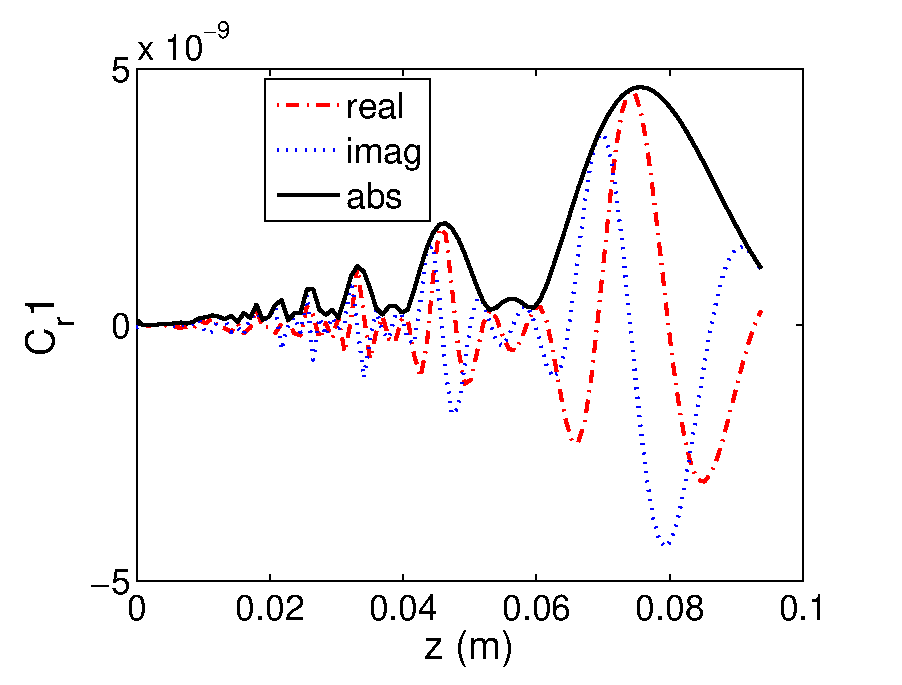
\includegraphics[scale=.44]{../media/Figs/Cr1}}
\end{minipage}%
\begin{minipage}{.5\linewidth}
\centering
\subfloat[$ \mathcal{C}_{r_\perp}(z) $ for $ r_\perp > a $]{\label{Czb}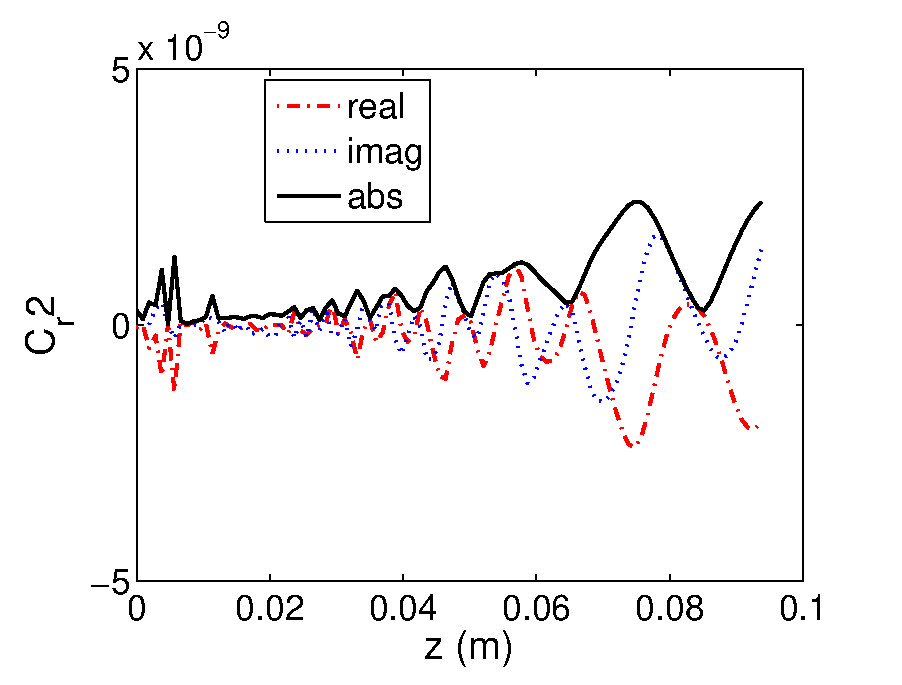
\includegraphics[scale=.44]{../media/Figs/Cr2}}
\end{minipage}
\par\medskip
\begin{minipage}{.5\linewidth}
\centering
\subfloat[$ \mathcal{C}_\phi(z) $ for $ r_\perp < a $]{\label{Czc}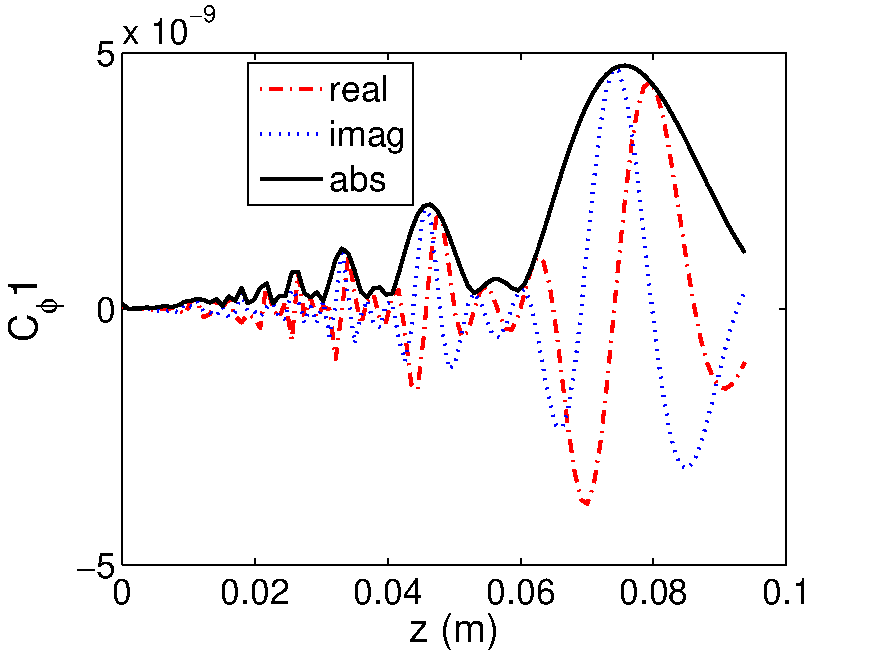
\includegraphics[scale=.44]{../media/Figs/Cphi1}}
\end{minipage}%
\begin{minipage}{.5\linewidth}
\centering
\subfloat[$ \mathcal{C}_\phi(z) $ for $ r_\perp > a $]{\label{Czd}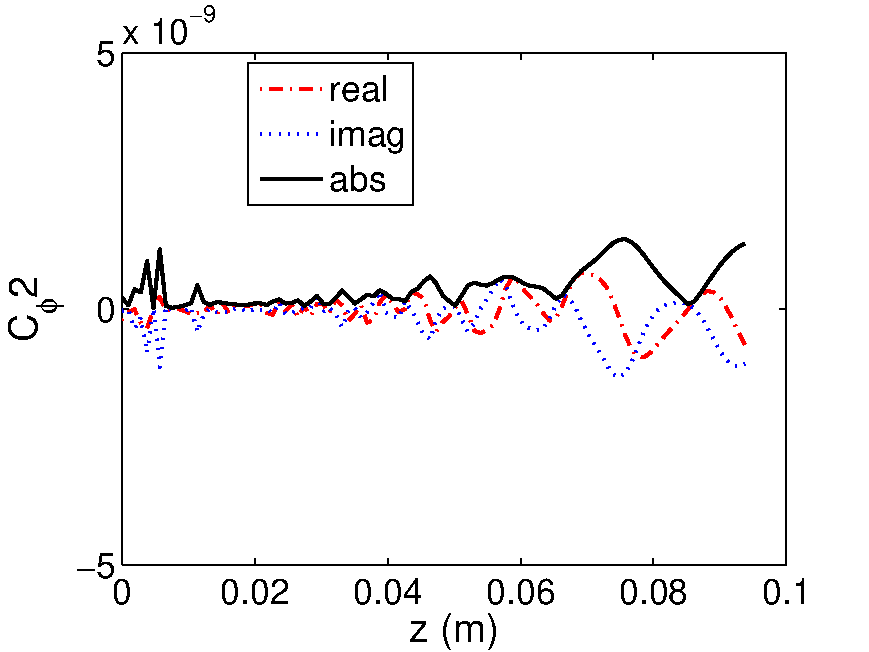
\includegraphics[scale=.44]{../media/Figs/Cphi2}}
\end{minipage}
\caption{$ \mathcal{C}^{(\omega,p=+,f=+)}(z) $. The values of these coefficients are in an arbitrary unit. }
\label{Cz}
\end{figure}




\begin{figure}[H] 
\centering
\subfloat[$ \mathcal{A}(z) $]{\label{Az}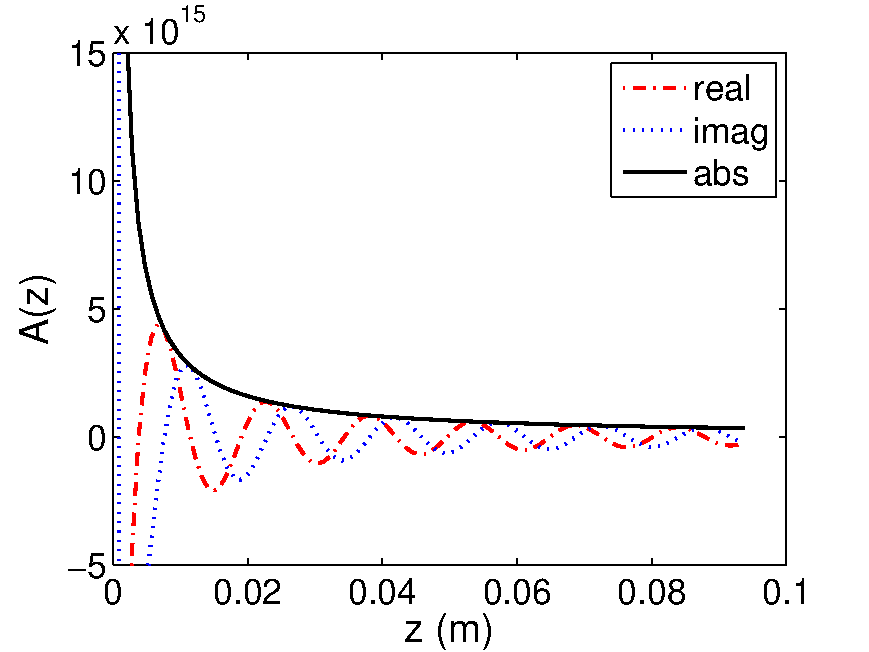
\includegraphics[scale=.5]{../media/Figs/Az}}
\par\medskip
\begin{minipage}{.5\linewidth}
\centering
\subfloat[$ \mathcal{C}_{r_\perp}(z) $]{\label{Crz}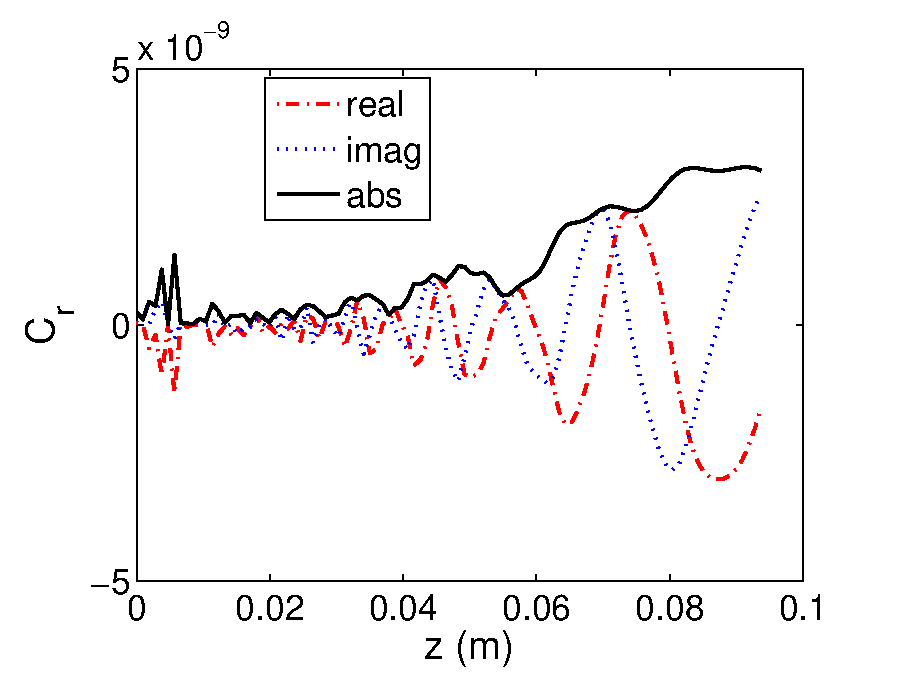
\includegraphics[scale=.44]{../media/Figs/Cr}}
\end{minipage}%
\begin{minipage}{.5\linewidth}
\centering
\subfloat[$ \mathcal{C}_\phi(z) $ ]{\label{Cphiz}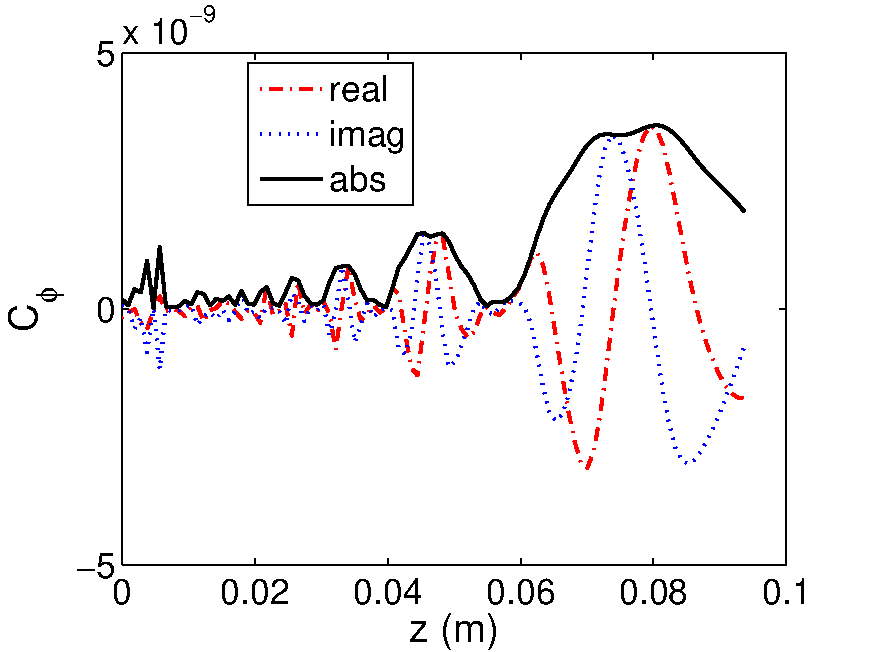
\includegraphics[scale=.44]{../media/Figs/Cphi}}
\end{minipage}
\par\medskip
\begin{minipage}{.5\linewidth}
\centering
\subfloat[$ \mathcal{S}_{r_\perp}(z) $ ]{\label{Srz}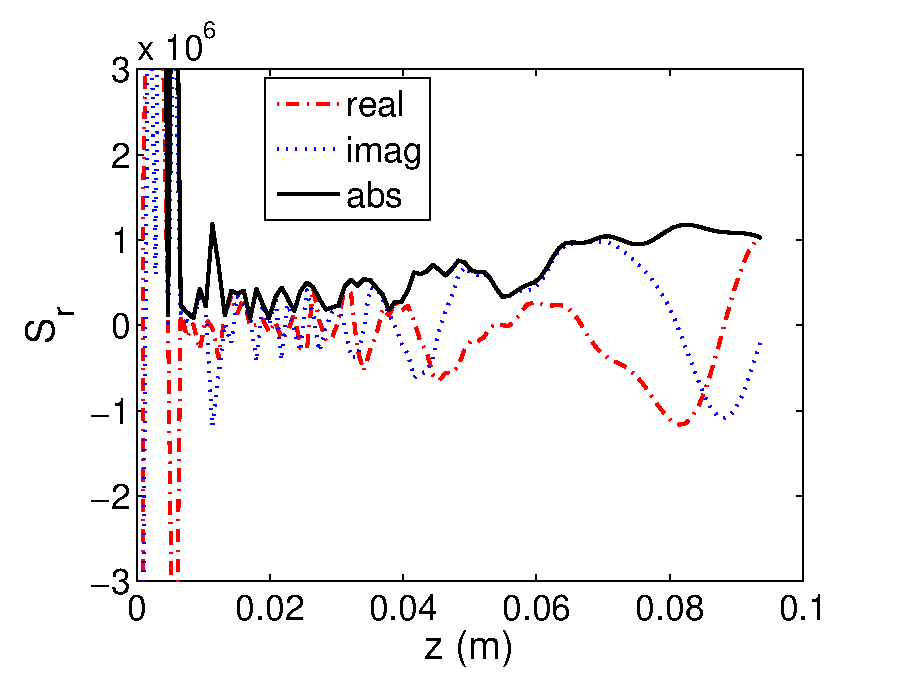
\includegraphics[scale=.44]{../media/Figs/Sr}}
\end{minipage}%
\begin{minipage}{.5\linewidth}
\centering
\subfloat[$ \mathcal{S}_\phi(z) $]{\label{Sphiz}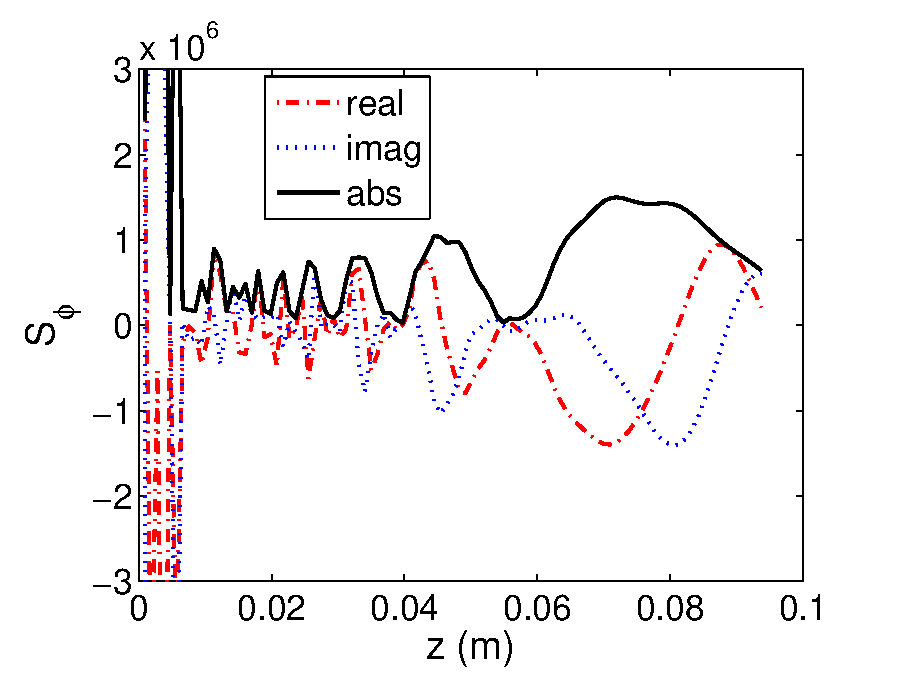
\includegraphics[scale=.44]{../media/Figs/Sphi}}
\end{minipage}
\caption{$ \mathcal{A}(z) $, $ \mathcal{C}^{(\omega,p=+,f=+)}(z) $ and $ \mathcal{S}^{(\omega,p=+,f=+)}(z) $. The values of these coefficients are in an arbitrary unit. There should be some fast chopping in $ \mathcal{A}(z) $ and $ \mathcal{S}^{(\mu)}(z) $. However, due to the cost of computing time, we did not give a fine enough calculation in our plots. See following plots for the calculation results with an improved resolution.  }
\label{ACSz}
\end{figure}


\scalefig{../media/Figs/InterferencePeriods}{0.6}{Wave path-difference of the interference between a monochromatic light emitted from a point atom located at $ \br'=(r'_\perp,\phi',z')=(2a,0,0) $ and a laser beam propagating along the $ z $-axis at the same wavelength $ \lambda_0=937.1 $ nm. The  horizontal axis of the plot is scaled in terms of the radium $ a $ of the nanofiber. The vertical axis is the wave path-difference measured along the laser's propagation direction of $ z $-axis, which is scaled by the wavelength $ \lambda=\lambda_0 $. As we can see, the interference period is uniform, and is on the order of $ 4.2a $.  This rough calculation implies that the chopping frequency in $ z $-direction should on the order of the wavelength, which should be reflected in Fig.~\ref{ACSz} and related plots. }


\newpage
Notice that, calculation resolution matters to the results. For comparison, we run the exact simulation as above but with a better $ z $-resolution.  The results are shown in Figs.~\ref{Cz_1} and~\ref{ACSz_1}. In $ z\in (0,1)\,\mathrm{mm} $ region, we calculate the coefficients in every $ 20 $ wavelengths; in $ z\in[2,100]\,\mathrm{mm} $ region, we calculate the coefficients in every $ \lesssim 1000 $ wavelengths. While in Figs.~\ref{Cz} and~\ref{ACSz} before, we calculate the coefficients evenly in every $ 1000 $ wavelengths. Also, when we calculated the integrals in the figures below, we used a $ 3 $ times better resolution in $ r_\perp\in(a,5a) $ region, which gives more detailed features of the $ \mathcal{C}^{(\mu)} (z)$ and $ \mathcal{S}^{(\mu)}(z) $ plots. With this improved resolution, it takes more than one hour to run the full calculation on a Thinkpad X200 laptop. 

\begin{figure}[H] 
\begin{minipage}{.5\linewidth}
\centering
\subfloat[$ \mathcal{C}_{r_\perp}(z) $ for $ r_\perp < a $]{\label{Cza_1}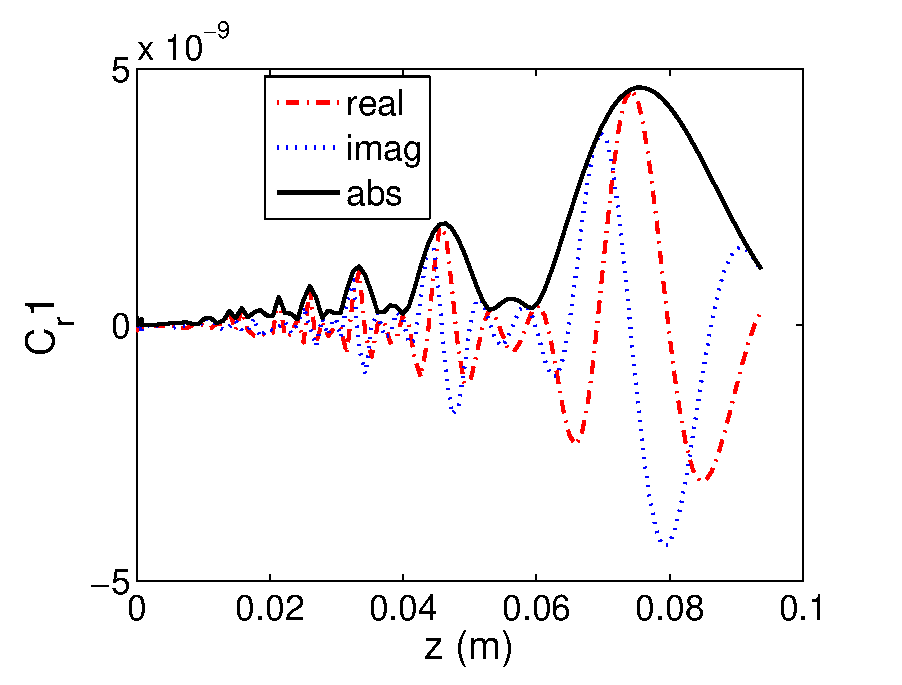
\includegraphics[scale=.44]{../media/Figs/Cr1_1}}
\end{minipage}%
\begin{minipage}{.5\linewidth}
\centering
\subfloat[$ \mathcal{C}_{r_\perp}(z) $ for $ r_\perp > a $]{\label{Czb_1}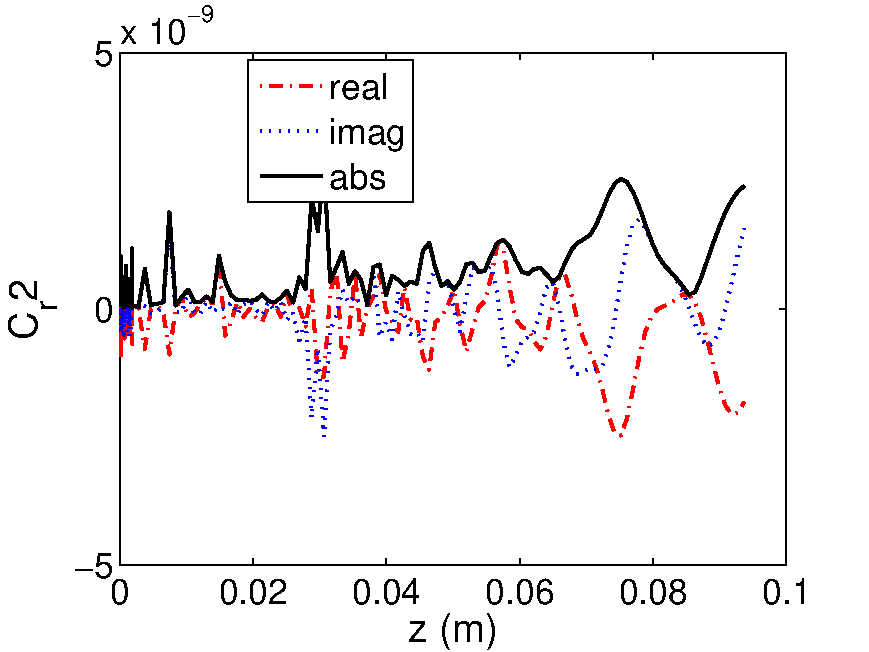
\includegraphics[scale=.44]{../media/Figs/Cr2_1}}
\end{minipage}
\par\medskip
\begin{minipage}{.5\linewidth}
\centering
\subfloat[$ \mathcal{C}_\phi(z) $ for $ r_\perp < a $]{\label{Czc_1}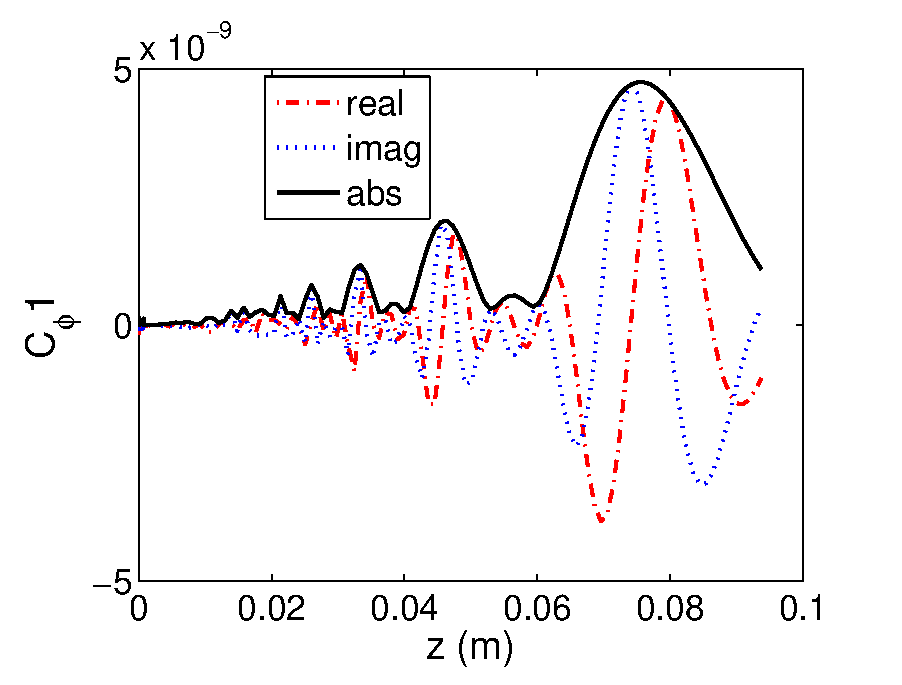
\includegraphics[scale=.44]{../media/Figs/Cphi1_1}}
\end{minipage}%
\begin{minipage}{.5\linewidth}
\centering
\subfloat[$ \mathcal{C}_\phi(z) $ for $ r_\perp > a $]{\label{Czd_1}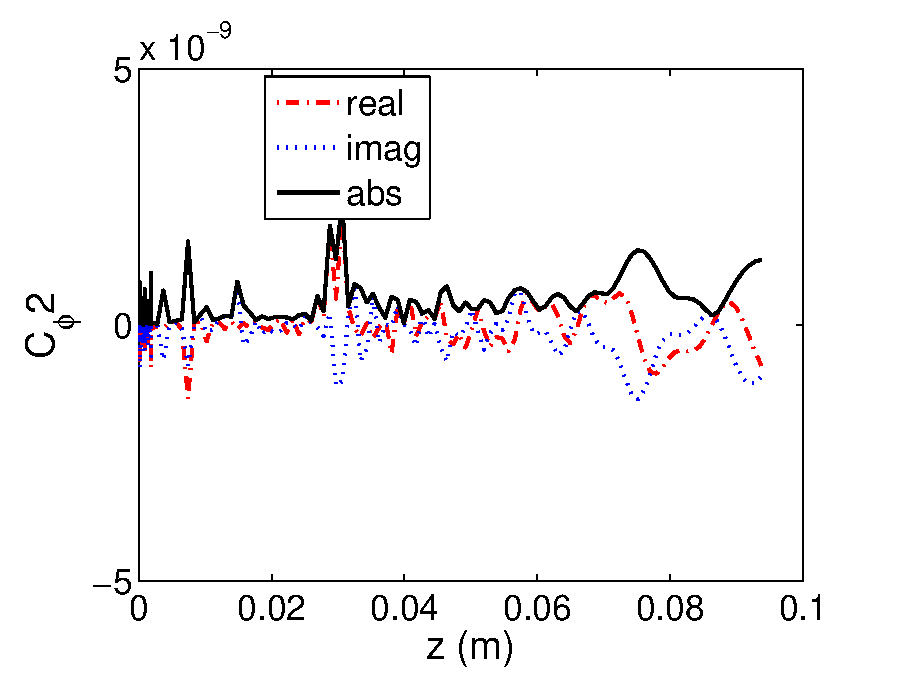
\includegraphics[scale=.44]{../media/Figs/Cphi2_1}}
\end{minipage}
\caption{$ \mathcal{C}^{(\omega,p=+,f=+)}(z) $. The values of these coefficients are in an arbitrary unit. Resolution is improved (see text).}
\label{Cz_1}
\end{figure}




\begin{figure}[H] 
\centering
\subfloat[$ \mathcal{A}(z) $]{\label{Az_1}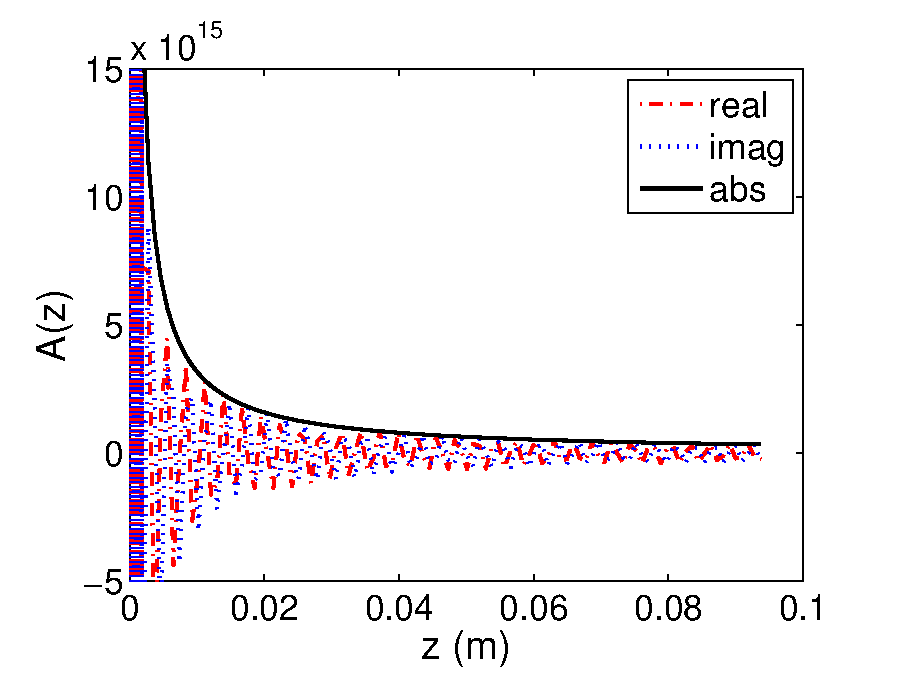
\includegraphics[scale=.5]{../media/Figs/Az_1}}
\par\medskip
\begin{minipage}{.48\linewidth}
\centering
\subfloat[$ \mathcal{C}_{r_\perp}(z) $]{\label{Crz_1}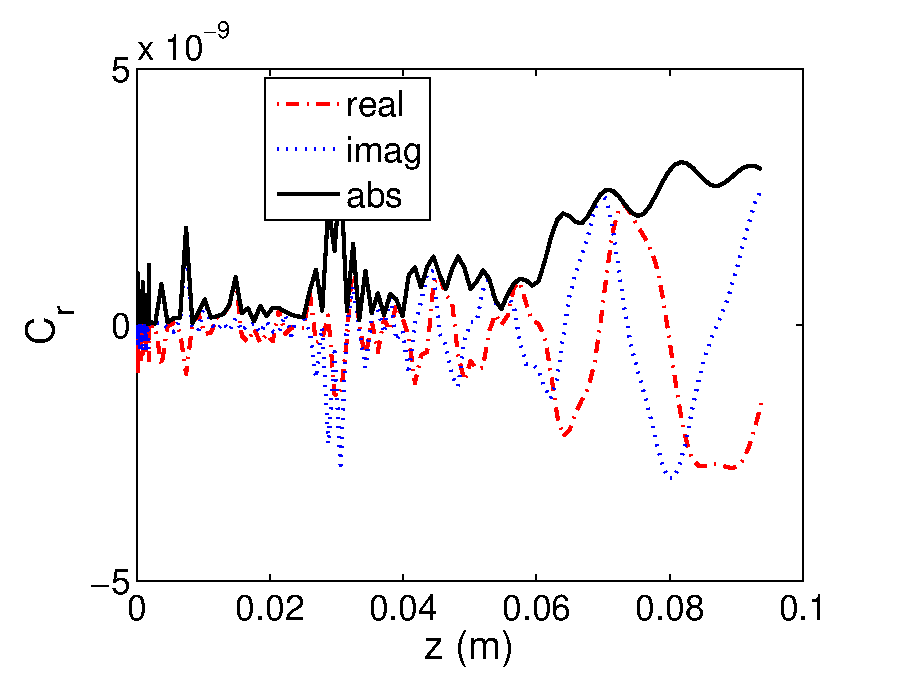
\includegraphics[scale=.42]{../media/Figs/Cr_1}}
\end{minipage}%
\begin{minipage}{.48\linewidth}
\centering
\subfloat[$ \mathcal{C}_\phi(z) $ ]{\label{Cphiz_1}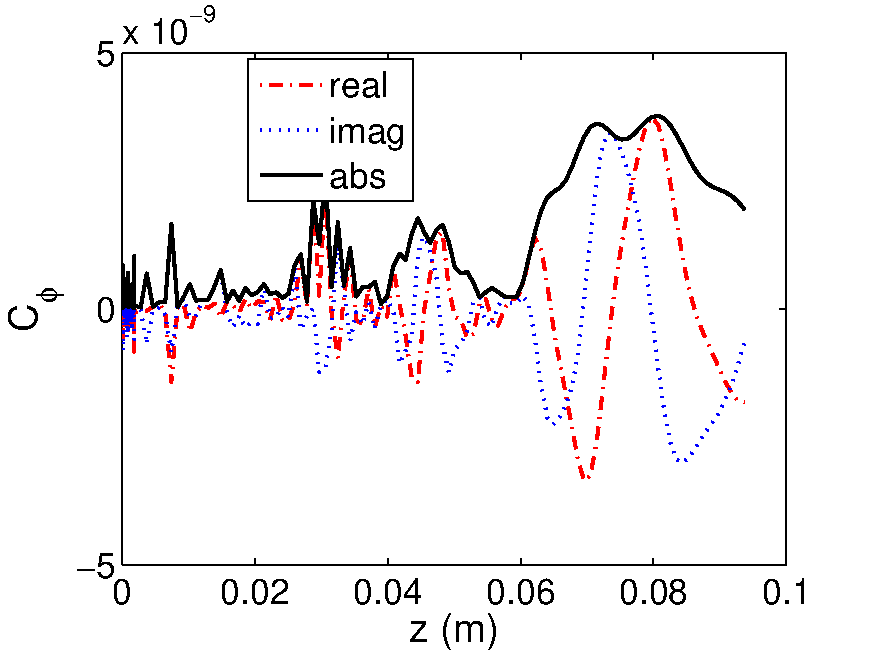
\includegraphics[scale=.42]{../media/Figs/Cphi_1}}
\end{minipage}
\par\medskip
\begin{minipage}{.48\linewidth}
\centering
\subfloat[$ \mathcal{S}_{r_\perp}(z) $ ]{\label{Srz_1}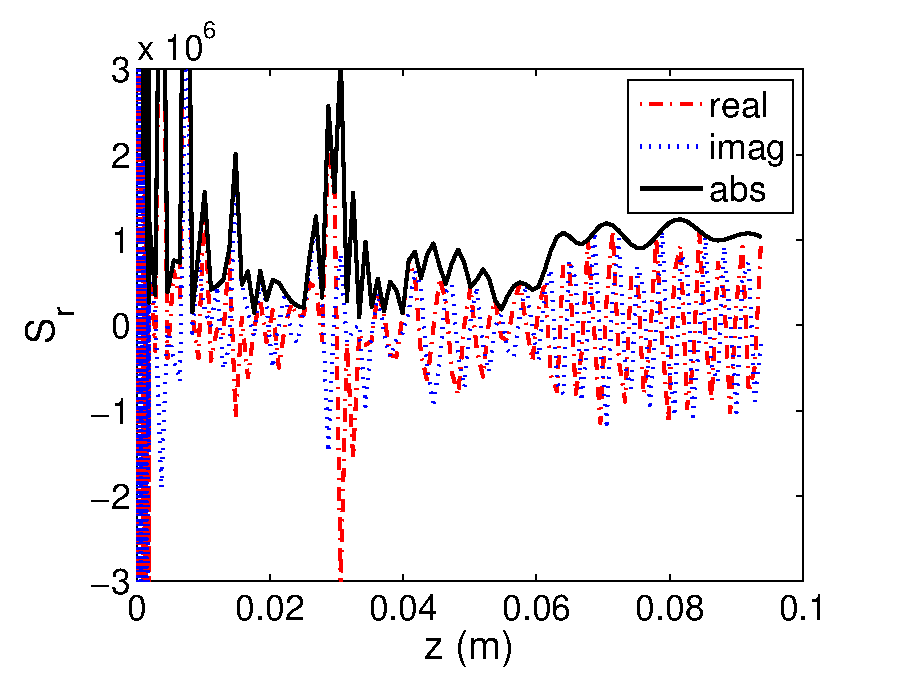
\includegraphics[scale=.42]{../media/Figs/Sr_1}}
\end{minipage}%
\begin{minipage}{.48\linewidth}
\centering
\subfloat[$ \mathcal{S}_\phi(z) $]{\label{Sphiz_1}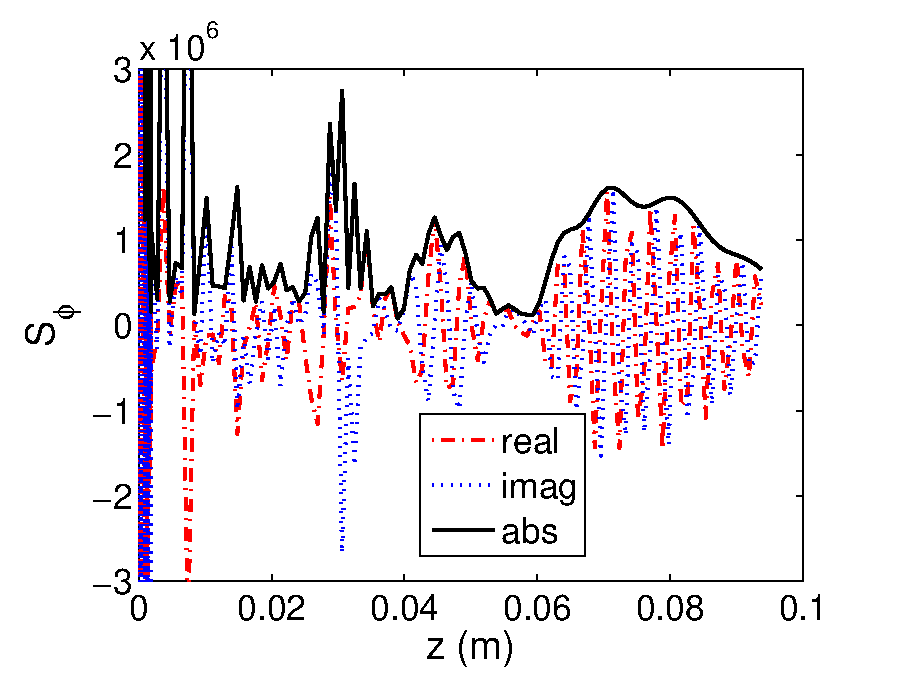
\includegraphics[scale=.42]{../media/Figs/Sphi_1}}
\end{minipage}
\caption{$ \mathcal{A}(z) $, $ \mathcal{C}^{(\omega,p=+,f=+)}(z) $ and $ \mathcal{S}^{(\omega,p=+,f=+)}(z) $. The values of these coefficients are in an arbitrary unit. Resolution is improved (see text).}
\label{ACSz_1}
\end{figure}
